\newpage

\section{heatmap logarithmic}

\begin{tikzpicture}
\begin{axis}[
scale=1,
/pgfplots/scale only axis,
/pgfplots/width=5cm,
/pgfplots/height=5cm,
colorbar,
colorbar style={ylabel={}},
colormap/viridis,
point meta max=51,
point meta min=0,
tick align=outside,
tick pos=left,
xmin=0-.5, xmax=10-.5,
ymin=0-.5, ymax=10-.5,
xtick={-0.5,4.5,9.5},
xticklabels={$0$,$0.5$,$1$},
ytick={-0.5,4.5,9.5},
yticklabels={$0$,$0.75$,$1.5$},
x label style={at={(axis description cs:0.5,-0.01)},anchor=north},
y label style={at={(axis description cs:+0.1,.5)},rotate=0,anchor=south},
xlabel={$foo$ [-]},
ylabel={$bar$ [-]},
]

\addplot graphics 
[includegraphics cmd=\pgfimage,xmin=-0.5, xmax=9.5, ymin=9.5, ymax=-0.5] 
{data/heatmap_log.png};

\end{axis}
\node at (8cm,2.5cm) [anchor=north , rotate=0] {$\log(N)$[-]};

\end{tikzpicture}

\subsection{how to}
\begin{itemize}
	\item preprocessing with python:
	\begin{itemize}
		\item import packages
	\begin{lstlisting}[language = python]
import numpy as np
import matplotlib.pyplot as plt
\end{lstlisting}
	\item transform rawdata to grid:
	\begin{lstlisting}[language = python]
def pos_in_grid(val, grid):
   pos = sum( [1 if x <= val else 0 for x in grid[1:-1] ] )
   return pos

def data_2_grid( filename, res_x, res_y ):

   with open("example_001.csv","r") as fp:
      x_data, y_data = np.loadtxt(fp,
                                  delimiter=' ',
                                  usecols=(0,1),
                                  unpack = True)

   x_grid = np.linspace( min(x_data), max(x_data), res_x+1 )
   y_grid = np.linspace( min(y_data), max(y_data), res_y+1 )

   grid = np.zeros((res_x, res_y))

   for x,y in zip(x_data, y_data):
      j = pos_in_grid(x, x_grid)
      i = pos_in_grid(y, y_grid)
      grid[i][j] += 1

   return grid
	\end{lstlisting}
	\item create png image
	\begin{lstlisting}
grid = data_2_grid("example_001.csv",15,15)
fig = plt.figure(frameon = False)
fig.set_size_inches(2,2)
ax = plt.Axes(fig, [0,0,1,1])
ax.set_axis_off()
fig.add_axes(ax)
ax.imshow(grid,  origin='lower')
fig.savefig("heatmap.png")
	\end{lstlisting}
	\end{itemize}

\item plot commands:

\begin{lstlisting}
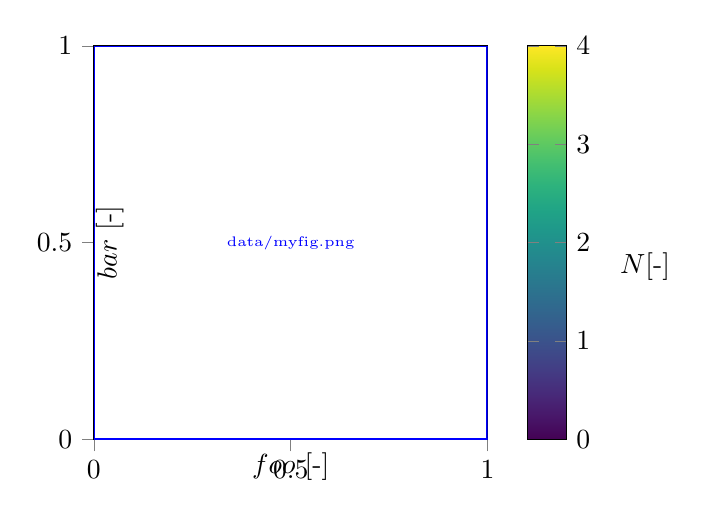
\begin{tikzpicture}
\begin{axis}[
scale=1,
/pgfplots/scale only axis,
/pgfplots/width=5cm,
/pgfplots/height=5cm,
colorbar,
colorbar style={ylabel={}},
colormap/viridis,
point meta max=4,
point meta min=0,
tick align=outside,
tick pos=left,
xmin=0-.5, xmax=10-.5,
ymin=0-.5, ymax=10-.5,
xtick={-0.5,4.5,9.5},
xticklabels={$0$,$0.5$,$1$},
ytick={-0.5,4.5,9.5},
yticklabels={$0$,$0.5$,$1$},
x label style={at={(axis description cs:0.5,-0.01)},anchor=north},
y label style={at={(axis description cs:+0.1,.5)},rotate=0,anchor=south},
xlabel={$foo$ [-]},
ylabel={$bar$ [-]},
]

\addplot graphics 
[includegraphics cmd=\pgfimage,xmin=-0.5, xmax=9.5, ymin=9.5, ymax=-0.5] 
{data/myfig.png};

\end{axis}
\node at (7cm,2.5cm) [anchor=north , rotate=0] {$N$[-]};

\end{tikzpicture}
\end{lstlisting}

\end{itemize}

